%% Figure 1: PhyNetPy architecture.
%%
%% Compiles standalone (tectonic -X compile figures/architecture.tex). Every
%% box corresponds to a module or subpackage under src/; the caption in
%% sections/architecture.tex names them.

\documentclass[border=6pt]{standalone}
\usepackage{tikz}
\usetikzlibrary{arrows.meta,positioning,fit,backgrounds}
% Defined in main.tex too; \providecommand keeps this file standalone-safe.
\providecommand{\code}[1]{\texttt{#1}}
\begin{document}
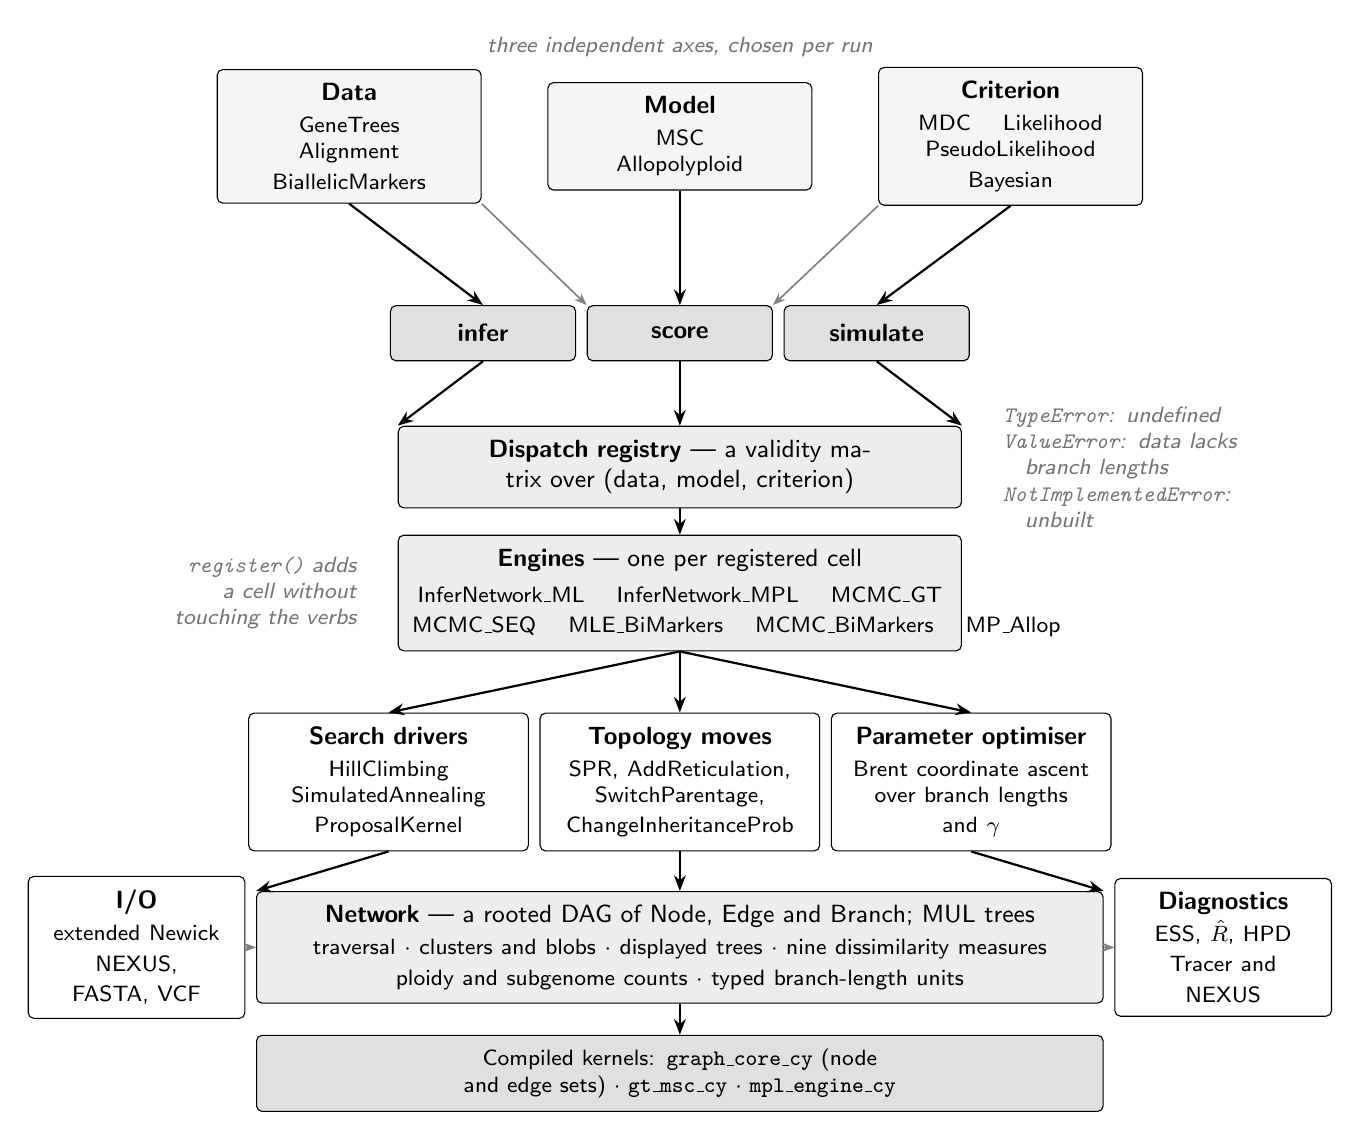
\begin{tikzpicture}[
  font=\sffamily\small,
  box/.style={
    draw, rounded corners=2pt, align=center, inner sep=5pt,
    minimum height=8mm
  },
  axis/.style={box, fill=black!4, text width=30mm},
  verb/.style={box, fill=black!12, text width=20mm,
               font=\sffamily\bfseries\small, minimum height=7mm},
  core/.style={box, fill=black!7},
  shared/.style={box, fill=white, text width=32mm},
  kernel/.style={box, fill=black!12, font=\sffamily\footnotesize},
  lbl/.style={font=\sffamily\footnotesize\itshape, text=black!55, align=left},
  flow/.style={-{Stealth[length=2mm]}, thick},
  rail/.style={-{Stealth[length=1.6mm]}, semithick, black!50},
]

% ---- the three axes -----------------------------------------------------
\node[axis] (data)      at (-4.2, 7.3) {\textbf{Data}\\[2pt]
  \footnotesize GeneTrees\\ Alignment\\ BiallelicMarkers};
\node[axis] (model)     at ( 0.0, 7.3) {\textbf{Model}\\[2pt]
  \footnotesize MSC\\ Allopolyploid\\[\baselineskip]};
\node[axis] (criterion) at ( 4.2, 7.3) {\textbf{Criterion}\\[2pt]
  \footnotesize MDC \quad Likelihood\\ PseudoLikelihood\\ Bayesian};

\node[lbl, above=2mm of model, text width=52mm, align=center]
  {three independent axes, chosen per run};

% ---- the verbs ----------------------------------------------------------
\node[verb] (infer)    at (-2.5, 4.8) {infer};
\node[verb] (score)    at ( 0.0, 4.8) {score};
\node[verb] (simulate) at ( 2.5, 4.8) {simulate};

\draw[flow] (data.south)      -- (infer.north);
\draw[flow] (model.south)     -- (score.north);
\draw[flow] (criterion.south) -- (simulate.north);
\draw[rail] (data.south east)      -- (score.north west);
\draw[rail] (criterion.south west) -- (score.north east);

% ---- registry -----------------------------------------------------------
\node[core, text width=68mm] (registry) at (0, 3.1)
  {\textbf{Dispatch registry} --- a validity matrix over
   (data, model, criterion)};

\draw[flow] (infer.south)    -- (registry.north west);
\draw[flow] (score.south)    -- (registry.north);
\draw[flow] (simulate.south) -- (registry.north east);

\node[lbl, right=4mm of registry, text width=33mm] {%
  \code{TypeError}: undefined\\
  \code{ValueError}: data lacks\\ \hphantom{xx}branch lengths\\
  \code{NotImplementedError}:\\ \hphantom{xx}unbuilt};

% ---- engines ------------------------------------------------------------
\node[core, text width=68mm] (engines) at (0, 1.5)
  {\textbf{Engines} --- one per registered cell\\[2pt]
   \mbox{\footnotesize InferNetwork\_ML \quad InferNetwork\_MPL \quad
   MCMC\_GT}\\
   \mbox{\footnotesize MCMC\_SEQ \quad MLE\_BiMarkers \quad
   MCMC\_BiMarkers \quad MP\_Allop}};
\draw[flow] (registry) -- (engines);

\node[lbl, left=4mm of engines, text width=26mm, align=right]
  {\code{register()} adds\\ a cell without\\ touching the verbs};

% ---- shared machinery ---------------------------------------------------
\node[shared] (search) at (-3.7, -0.9)
  {\textbf{Search drivers}\\[2pt]
   \footnotesize HillClimbing\\ SimulatedAnnealing\\ ProposalKernel};
\node[shared] (moves) at (0, -0.9)
  {\textbf{Topology moves}\\[2pt]
   \footnotesize SPR, AddReticulation,\\ SwitchParentage,\\ ChangeInheritanceProb};
\node[shared] (optim) at (3.7, -0.9)
  {\textbf{Parameter optimiser}\\[2pt]
   \footnotesize Brent coordinate ascent\\ over branch lengths\\ and $\gamma$};

\draw[flow] (engines.south) -- (search.north);
\draw[flow] (engines.south) -- (moves.north);
\draw[flow] (engines.south) -- (optim.north);

% ---- network core -------------------------------------------------------
\node[core, text width=104mm] (net) at (0, -3.0)
  {\textbf{Network} --- a rooted DAG of Node, Edge and Branch; MUL trees\\[2pt]
   \footnotesize traversal $\cdot$ clusters and blobs $\cdot$ displayed trees
   $\cdot$ nine dissimilarity measures\\
   \footnotesize ploidy and subgenome counts $\cdot$ typed branch-length units};

\draw[flow] (search.south) -- (net.north west);
\draw[flow] (moves.south)  -- (net.north);
\draw[flow] (optim.south)  -- (net.north east);

% ---- compiled kernels ---------------------------------------------------
\node[kernel, text width=104mm] (cy) at (0, -4.6)
  {Compiled kernels: \code{graph\_core\_cy} (node and edge sets)
   $\cdot$ \code{gt\_msc\_cy} $\cdot$ \code{mpl\_engine\_cy}};
\draw[flow] (net) -- (cy);

% ---- side rails ---------------------------------------------------------
\node[shared, text width=24mm] (io) at (-6.9, -3.0)
  {\textbf{I/O}\\[2pt]
   \footnotesize extended Newick\\ NEXUS, FASTA, VCF};
\draw[rail] (io.east) -- (net.west);

\node[shared, text width=24mm] (diag) at (6.9, -3.0)
  {\textbf{Diagnostics}\\[2pt]
   \footnotesize ESS, $\hat{R}$, HPD\\ Tracer and NEXUS};
\draw[rail] (net.east) -- (diag.west);

\end{tikzpicture}
\end{document}
